\newSec[PrincGRASP]{GRASP}{2}

\newSec[PrincGRASPKopp]{Kopplung}{3}
Der Einsatz von \ROS\ deutet an dieser Stelle auf eine lose Kopplung hin (siehe \refCap{MusterObserver}).\footnote{vgl. Vorlesungsfolien \glq Programming Principles\grq (Seite 50)} 

Durch polymorphe Methodenaufrufe liegt eine mäßige Kopplung vor. Dies wurde in der \CodeClass{ControllerSystem} der \CodeMeth{addController} umgesetzt.\\
\href{https://github.com/MobMonRob/ROSLabDrohne/blob/8b5d30dbdfbd41a7e10fa8d512db42cad5bb6d16/Code/Controller/include/Controller/ControllerSystem.h\#L28}{Link: Controller/ControllerSystem.h\#L28 ff.}


Abgesehen von den genannten Punkten ist der zugrundeliegende Code eher stark gekoppelt, da häufig statische Methodenaufrufe sowie Methodendefinitionen verwendet werden.


\newSec[PrincGRASPKopp]{Kohäsion}{3}
An einem Beispiel (siehe \refImg{fig:Cohe}) wird der technische Ansatz dargestellt:\\
Methoden werden mit Attributen assoziiert und anschließend bewertet, inwiefern die Attribute der Klasse interagieren.

\begin{figure}[ht!]
\vspace{0.25cm}
\begin{center}
\fbox{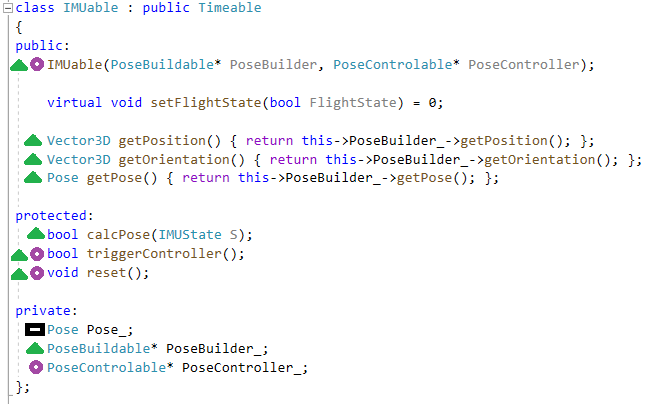
\includegraphics[width=15cm]{Pictures/Cohesion_IMUable.png}}
\caption{Kohäsion am Beispiel der Klasse IMUable}
\label{fig:Cohe}
\end{center}

\vspace{0.25cm}
In \refImgShort{fig:Cohe} werden Methoden zu Attributen zugeordnet, um den Grad der Kohäsion bestimmen zu können.\\
Es zeigt sich, dass die \CodeVar{Pose\_} nicht innerhalb der Klasse verwendet wird. Somit könnte dieses Attribut entfernt werden.\\
Die verbleibenden Attribute sind über Methoden miteinander verbunden und bilden somit eine hohe Kohäsion ab.
\end{figure}









